\documentclass[final,5p,times]{elsarticle}
\usepackage[T1]{fontenc}
\usepackage[utf8]{inputenc}
\usepackage{amsmath,amssymb,amsthm,booktabs,array,graphicx,microtype}
\usepackage{xcolor}
\usepackage{xurl}
\usepackage[hidelinks]{hyperref}
\usepackage{balance}
\journal{Neurocomputing}
\newtheorem{proposition}{Proposition}
\newcommand{\SSmodel}{StableShift}
\newcommand{\R}{\mathbb{R}}
\setlength{\tabcolsep}{4pt}
\setlength{\emergencystretch}{1.5em}
\renewcommand{\dbltopfraction}{0.95}
\renewcommand{\textfraction}{0.03}
\setcounter{dbltopnumber}{2}
\begin{document}
\begin{frontmatter}
\title{Anchored electricity-demand forecasting with bounded label-free adaptation}
\author[bjtu]{Yanbo Bian\corref{cor1}}
\ead{24722081@bjtu.edu.cn}
\cortext[cor1]{Corresponding author.}
\affiliation[bjtu]{organization={Computer Science and Technology, Weihai International Academy, Beijing Jiaotong University},city={Weihai},country={China}}
\begin{abstract}
Electricity-demand forecasting requires models to preserve recurring structure while responding to changing observations. We introduce StableShift, an anchored forecaster that separates a seasonal reference, learned linear and neural corrections, and a low-rank online state. A frozen temporal encoder supplies features to a 2,048-parameter adapter, which receives at most one label-free reconstruction update per forecast origin. A sensitivity bound links the projected update to its forecast displacement. Five-seed experiments evaluate 24 h and 168 h forecasts on EIA-930 observations through June 2026 and historical ECL and Ausgrid benchmarks. On the 2026 EIA-930 holdout, StableShift reduces 24 h mean absolute error by 5.1\% relative to validation-selected TiDE, with a pointwise paired 95\% confidence interval of 1.2--8.7\% improvement. Its advantage reaches 19.7\% under the specified block-anomaly perturbation. Chronological comparisons favor the selected baselines on ECL and Ausgrid. Matched interventions locate the EIA gains primarily in the learned corrections: disabling online updates changes mean absolute error by less than 0.053\% across all main conditions. Together, these results support accurate regional forecasting and an explicit separation between learned forecast corrections and bounded online modification.
\end{abstract}
\begin{keyword}
Electricity-demand forecasting \sep Distribution shift \sep Test-time adaptation \sep Temporal convolution \sep Low-rank learning \sep Forecast sensitivity
\end{keyword}
\end{frontmatter}

\section{Introduction}
An electricity-demand forecast connects recent observations to decisions that extend beyond them. A day-ahead estimate must resolve the next daily cycle; a week-ahead estimate must also accommodate changes in weather, activity and calendar phase. Recent work continues to develop models around these operational horizons, including multi-horizon building-demand systems and compact neural forecasters \cite{baydan2026operational,forootani2026compact}. The central challenge is therefore not simply to represent a long history. It is to determine which features of that history should persist into the forecast and which should be revised when new observations arrive.

Modern forecasting architectures approach this problem through different inductive biases. Linear decomposition makes temporal structure directly accessible \cite{zeng2023transformers}; patch-based attention, temporal variation modeling, variable-wise attention and dense encoders provide richer representations \cite{nie2023patchtst,wu2023timesnet,liu2023itransformer,das2023tide}. These developments have broadened the available model family substantially \cite{liao2026survey}. Their performance nevertheless depends on the relationship between the training distribution and the deployment stream. Normalization, calibration and adaptation address different parts of this relationship \cite{liu2022nonstationary,fan2023dishts,chen2024calibration}. Work in 2026 further explores prototype-based shift modeling, neural-ODE adaptation and optimization under distribution change \cite{apt2026,adanodes2026,adamshift2026}.

Adaptive forecasting systems couple two sources of performance: the representation learned before deployment and the changes made as observations arrive. Resolving their contributions requires measuring forecast accuracy alongside the marginal effect of online updates. Paired deployment streams make this distinction directly observable, connecting a self-supervised update on the context to its effect on future-load error. This question is particularly consequential for long horizons, where the labels needed to evaluate an update arrive only after a substantial delay.

We study this distinction with an architecture that makes its components directly accessible. StableShift predicts a correction to an explicit seasonal reference. Its temporal encoder and forecasting head remain fixed at deployment; only two low-rank factors can change online. A drift gate triggers one masked-reconstruction step using the already observed context. This arrangement creates two experimentally separable questions: whether the learned forecaster improves on strong fixed baselines, and whether updating its small online state provides an additional benefit. A same-context sensitivity bound connects the update size to its possible effect on the forecast.

The study makes three contributions. First, it formulates a seasonal-reference forecasting architecture with a clearly delimited online learning pathway and a sensitivity result for that pathway. Second, it evaluates this design on a recent regional-demand holdout, observations from January--June 2026, alongside customer and household benchmarks with identical within-dataset evaluation rules. Third, it uses matched deployment interventions to separate the contributions of learned corrections, input conditioning, representation penalties and online updates. The evidence identifies a regional forecasting advantage and shows that its dominant source is the learned correction. This yields a more precise account of adaptive forecasting than accuracy or adaptation activity considered alone.

\section{Related work}
\subsection{Structured and non-stationary forecasting}
Temporal decomposition remains a strong foundation for forecasting. DLinear demonstrates the competitiveness of simple temporal mappings \cite{zeng2023transformers}; recent approaches extend decomposition through adaptive scales, multiresolution mixing and clustering \cite{hu2025adaptive,murad2025wpmixer,qiu2025duet}. PatchTST, TimesNet, iTransformer and TiDE represent complementary ways to model temporal and cross-variable structure \cite{nie2023patchtst,wu2023timesnet,liu2023itransformer,das2023tide}. Our architecture uses a shared linear decomposition correction alongside a temporal convolutional representation. The seasonal reference provides an explicit output coordinate system for these corrections.

Distribution-aware forecasting includes restoring non-stationary information after normalization, using separate normalization treatments across input and output distributions, and detecting context-driven calibration changes \cite{liu2022nonstationary,fan2023dishts,chen2024calibration}. Transitional shift across and within series has also motivated robust multivariate models \cite{he2025robust}. The 2026 APT framework and work on optimization under distribution shifts add further nearby alternatives \cite{apt2026,adamshift2026}. StableShift complements these approaches by separating a forecaster's fixed and mutable components and measuring their contributions through matched interventions.

\subsection{Test-time adaptation and constrained updates}
Test-time adaptation updates a trained model using deployment observations. Continual adaptation studies the accumulation of such changes across a stream \cite{wang2022continualtta}. Forecasting-specific methods address non-stationarity through test-time learning \cite{kim2025tta}, including the recent AdaNODEs approach \cite{adanodes2026}. StableShift uses masked reconstruction of past loads as its online objective. Future load labels never enter that objective.

Low-rank parameterizations provide a compact space for adaptation \cite{hu2021lora,ding2023peft}. Spectral normalization supplies a complementary control on learned weight matrices \cite{miyato2018spectral}. We combine a low-rank state with a projected update and derive a same-context sensitivity bound for the resulting forecast displacement.

\subsection{Electricity-demand evaluation}
Transfer across electricity consumers and regions introduces differences in scale and recurring structure \cite{antoniadis2024hierarchical}. ECL and Ausgrid offer customer- and household-level observations \cite{uci2015ecl,ratnam2015ausgrid}; EIA-930 provides a current regional operating-data source \cite{eia9302026}. A common evaluation framework is essential because data processing, model selection and evaluation windows can materially affect model rankings \cite{qiu2024tfb}. We retain original measurement units and evaluate chronological forecasting, controlled input perturbations and regional transfer separately. Secondary analyses report their available seed counts.

\section{Anchored forecasting with a small online state}
\subsection{Forecasting problem}
Let $x_t\in\R^{L\times(d+6)}$ contain the $L=336$ hours immediately preceding forecast origin $t$. The first $d$ channels are observed loads standardized using training statistics. The remaining channels are sine and cosine encodings of hour, weekday and day of year. The target $y_t\in\R^{H\times d}$ contains the next $H$ hours, with $H\in\{24,168\}$ in the main comparison. All outputs are direct multi-step point forecasts.

The forecaster has fixed parameters $\theta$ and an online state $\phi_t=(U_t,V_t)$. At each origin it first computes a context-only drift score, optionally updates $\phi_t$, and then issues the forecast. State persists across successive origins. Labels enter only the subsequent evaluation of issued forecasts. Figure~\ref{fig:method} summarizes the information flow.

\begin{figure*}[t]
\centering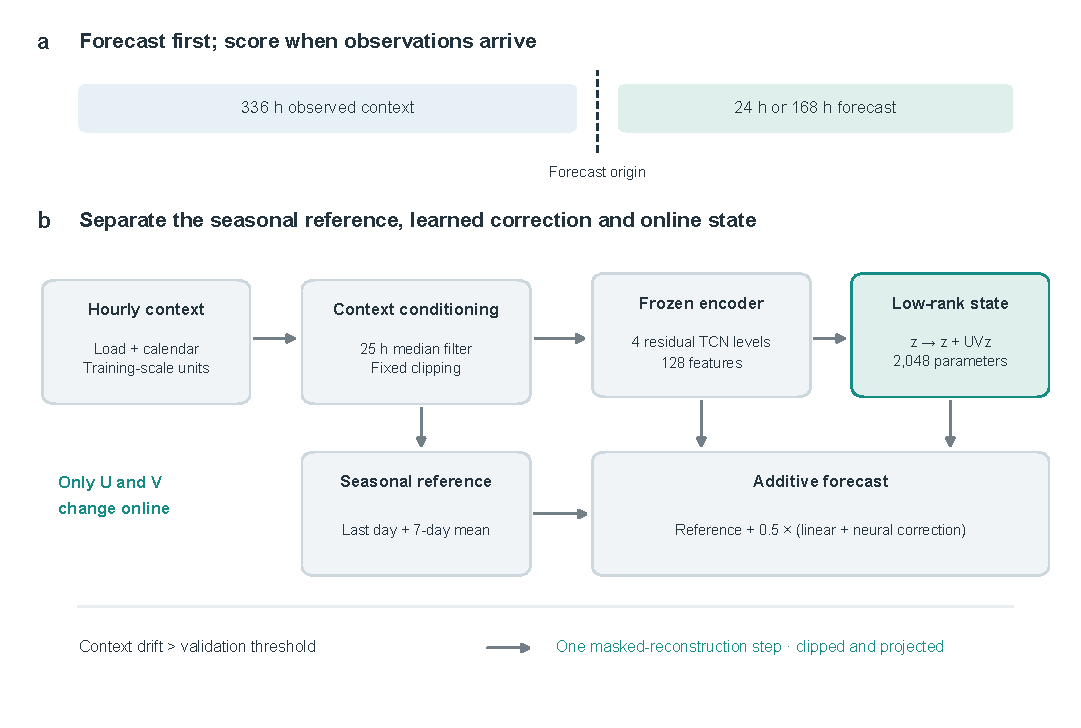
\includegraphics[width=\textwidth]{figures/fig1_architecture.pdf}
\caption{\textbf{An explicit boundary between forecasting knowledge and online modification.} (a) Each forecast uses the preceding 336 observed hours. Future labels enter scoring after issuance. (b) Context conditioning feeds a frozen temporal encoder and a seasonal reference. Learned linear and neural corrections augment that reference. Only the two low-rank factors are mutable during deployment. A validation-calibrated drift gate permits one masked-reconstruction step per origin. The diagram is schematic; all computations are detailed in the Methods and Supplementary Information.}
\label{fig:method}
\end{figure*}

\subsection{Seasonal reference and learned corrections}
Write $\widetilde x_t$ for the conditioned load context. A 25 h local median filter replaces observations beyond six local median absolute deviations, using a standardized deviation floor of 0.20. Values are then clipped to $[-6,6]$. The filter uses only the context available at the forecast origin. Calendar channels are retained unchanged.

For each daily position, a learned scalar $\alpha=\operatorname{sigmoid}(a)$ mixes the last observed daily cycle with the average of the preceding seven daily cycles:
\begin{equation}
 b_t=(1-\alpha)\widetilde x_{t-24:t}
 +\frac{\alpha}{7}\sum_{j=1}^{7}\widetilde x_{t-24j:t-24(j-1)}.
\end{equation}
The reference $s_t$ repeats $b_t$ to length $H$. The initial mixing weight is 0.6. A 24-point moving average decomposes the conditioned 336 h load context into a trend and a residual. Two learned temporal maps, shared across load channels, produce their combined correction $c_t^{\rm lin}$.

The neural encoder projects the input to width 128 and applies four residual levels with dilations $1,2,4,8$. Each level contains two kernel-three causal convolutions, per-time-step LayerNorm and GELU, with dropout 0.1. Flattened convolution-kernel matrices are spectrally normalized to a bound of one. The convolutional receptive field is 61 processed time steps; the seasonal and linear paths retain access to the full context.

Let $z_t\in\R^{128}$ be the last encoder feature, $p_t$ its learned stable projection, and $r_t$ a learned embedding of the most recent 24 h of load. A rank-eight adapter gives
\begin{equation}
 d_t=(I+UV)z_t,\qquad U\in\R^{128\times8},\quad V\in\R^{8\times128}.
\end{equation}
A two-layer GELU head $g_\theta$ combines these features:
\begin{equation}
 \widehat y_t=s_t+\rho\{c_t^{\rm lin}+g_\theta([p_t,d_t,r_t])\},\quad \rho=0.5.
 \label{eq:forecast}
\end{equation}
The temporal maps and final neural output layer are initialized to zero, so training begins from the mixed seasonal reference. The learned corrections are evaluated jointly in the anchor-only intervention.

\subsection{Offline learning and label-free deployment}
Offline learning minimizes
\begin{equation}
 \mathcal L=\mathcal L_{\rm pred}
 +0.05\mathcal L_{\rm cons}
 +0.0005\mathcal L_{\rm energy}
 +0.05\mathcal L_{\rm rec}.
\end{equation}
The prediction term is mean squared error in standardized units. The consistency term compares stable feature sequences for the original context and a copy with Gaussian load noise of standard deviation 0.01. Dropout remains active during training. The energy term penalizes the mean squared magnitude of the final stable feature. The reconstruction term predicts randomly masked load entries, using a 15\% mask; known calendar features remain available, and originally missing observations are excluded from this loss.

The drift score measures the magnitude of the context's mean standardized load:
\begin{equation}
 D(x_t)=\left(\frac1d\sum_{j=1}^{d}
 \left[\frac1L\sum_{\tau=1}^{L}x_{t,\tau,j}\right]^2\right)^{1/2}.
\end{equation}
Its threshold is the 95th percentile over eligible validation contexts. When the score exceeds the threshold, a deterministic origin-specific mask defines one reconstruction update on $U,V$. All other parameters remain frozen. The step uses learning rate 0.01, joint gradient norm clipping at one, and projection of each factor onto a Frobenius-norm ball of radius eight. Encoded masked features are detached before differentiation. The updated state is then used to forecast the unmasked observed context. Neither the input-condition label nor future loads are supplied to the deployment rule.

\subsection{Sensitivity of the mutable pathway}
For a fixed context, collect the unchanged terms of Eq.~\ref{eq:forecast} into $a(x)$ and $c(x)$, giving
\begin{equation}
 f_{U,V}(x)=a(x)+\rho W_o\sigma\{c(x)+W_d(I+UV)z(x)\}.
\end{equation}
Here $W_d$ is the adapter-feature block of the head's first weight matrix, $W_o$ is its output matrix, and $\sigma$ is GELU.

\begin{proposition}
Let $n=Hd$, and compare two adapter states at the same context, with dropout disabled. Their coordinate-averaged forecast displacement satisfies
\begin{align}
 \frac{\|f_{U',V'}(x)-f_{U,V}(x)\|_1}{n}
 &\leq K(x)\|U'V'-UV\|_2,\\
 K(x)&=\frac{\rho L_\sigma}{\sqrt n}\|W_o\|_2\|W_d\|_2\|z(x)\|_2,
\end{align}
where $L_\sigma=1.129$. If both states lie in the radius-$R$ factor balls, their matrix-product change is bounded by $R(\|U'-U\|_F+\|V'-V\|_F)$. A projected step from inside these balls, with learning rate $\eta$ and clipped joint gradient norm $G$, bounds that change by $\sqrt2R\eta G$.
\end{proposition}

Supplementary Section S1 gives the proof. The bound quantifies adaptation-induced displacement in standardized forecasts at a fixed context; conversion to original units includes the output scale matrix. Paired online/no-update streams measure the update's effect on forecast error.

\section{Experimental design}
\subsection{Recent regional data and cross-scale benchmarks}
EIA-930 contains seven balancing-authority regions: PJM, MISO, CISO, NYIS, ISNE, ERCO and SWPP. The prepared series spans 30,648 hourly observations from 1 January 2023 to 1 July 2026. We use reported observed demand in MW, train on 2023--2024, select models on 2025 and evaluate on January--June 2026 \cite{eia9302026}. Thus the most recent data provide a temporally separated operating-data evaluation.

Two historical benchmarks assess the same architecture at different aggregation scales. ECL uses the first 16 indexed customers, MT\_001--MT\_016, from 2011--2014, with each hour formed by averaging four quarter-hour power readings in kW \cite{uci2015ecl}. Ausgrid uses general-consumption readings for customers 001--016 from July 2010 to June 2013; two half-hour energy readings are summed to hourly energy in kWh \cite{ratnam2015ausgrid}. Their chronological training, validation and test proportions are 70/10/20. These are fixed indexed subsets, and the historical observation periods are retained in reporting.

All datasets preserve the hourly time grid. Input gaps are forward-filled from past observations. Normalization and daily-lag MASE denominators use observed training data only. Training and validation windows require complete observed future targets. During deployment every scheduled origin is processed, including origins whose targets later prove incomplete; only complete target blocks are scored. The six main cells contain respectively 169/181 and 19/25 scored/scheduled EIA origins, 292/292 and 41/41 ECL origins, and 180/219 and 25/31 Ausgrid origins. Exact timestamps, preprocessing and counts appear in Supplementary Section S2.

\subsection{Baselines, selection and deployment interventions}
Baselines are daily and weekly persistence, DLinear, PatchTST, TimesNet, iTransformer and TiDE. Neural baselines use the reference Time-Series-Library implementation pinned to a recorded commit, with width 64 and two encoder layers where applicable. All methods receive the same eligible context and target windows; wrappers supply calendar features to architectures that consume them. TiDE's scalar-output LayerNorm is replaced by an identity map to retain input dependence. Supplementary Section S3 records this implementation detail and all model settings.

Each trainable model receives two learning-rate trials, $10^{-3}$ and $3\times10^{-4}$, using AdamW, weight decay $10^{-4}$, batch size 32, at most 30 epochs and patience six. Training origins advance by 6 h and validation origins by 24 h. Checkpoints and the final trial are selected by original-unit validation MAE. Test origins advance by the forecast horizon. The main analysis uses seeds 11, 22, 33, 44 and 55. TimesNet has five completed seeds for EIA 24 h; its other available results, the three-seed EIA 48 h evaluation and partial archival PJM runs are reported separately. Main comparisons require five completed seeds for the method and cell concerned.

One reference comparator per dataset/horizon is selected by mean validation MAE among the completed five-seed baselines. This selects TiDE except for ECL 168 h, where it selects weekly persistence. The comparator remains fixed across input conditions. Daily and weekly persistence are deterministic; repeated seed identifiers do not imply independent fitted models.

Four interventions examine StableShift. \emph{Anchor only} retains its learned seasonal mixing weight and input conditioning but removes both corrections. \emph{No update} uses the same checkpoint without online modification. \emph{No filter} removes both median filtering and clipping while retaining the online gate. \emph{No representation penalties} retrains without the consistency and energy terms, retaining spectral normalization and reconstruction. Each condition begins from its selected checkpoint with a fresh state; origins within a condition remain chronological.

\subsection{Input perturbations and regional transfer}
The unmodified chronological holdout measures forecasting on observed future data. Four controlled conditions alter context loads only: 10\% independent missing inputs replaced by the training mean; a $1.35\times$ scaling of the last 14 standardized hours; an affine change $1.15x+0.10$ across the context; and a 28 h middle-context anomaly of signed magnitude four channelwise context standard deviations. Calendar features and future labels remain unchanged. These conditions measure response to altered observations, rather than simulating a joint change in future demand. A separate natural-shock indicator uses the training 95th percentile of mean absolute hourly context differences. Eligible counts are reported in the supplement.

A secondary regional-transfer experiment trains a shared univariate model on PJM, MISO, CISO, NYIS and ISNE and evaluates previously unseen ERCO and SWPP at 168 h, using three seeds. Held-out normalization is initialized from the 336 h preceding the first 2026 forecast and then frozen. Model selection and the drift threshold use only the five training regions. Historical held-out observations are used solely to calculate the evaluation MASE denominator. The available transfer baselines are daily and weekly persistence, DLinear and PatchTST.

\subsection{Metrics and uncertainty}
MAE averages absolute errors over scored origins, horizons, channels and seeds. RMSE is the square root of pooled squared error, and MASE scales channel errors by their training daily-lag absolute difference. We report input-degradation ratios relative to each method's unmodified error, together with paired differences from the validation-selected comparator.

Confidence intervals use 5,000 paired bootstrap resamples crossing common seed draws with common circular time blocks. Missing score slots remain on the deployment grid. The principal block spans at least seven days: seven 24 h origins or one 168 h origin. Sensitivity analyses use 14- and 28-day blocks. Intervals are pointwise percentile 95\% intervals. Null-centered bootstrap tests use an add-one Monte Carlo correction, followed by Holm adjustment across the 60 main MAE/RMSE comparisons; MASE and intervention families are adjusted separately. Joint calendar-day resampling gives equal-cell macro and worst-cell relative errors. This retains the dependence between horizons and conditions within each dataset. Supplementary Section S4 provides the full specification and numerical tables.

\section{Results}
\subsection{An advantage on the 2026 regional holdout}
StableShift achieves EIA-930 MAE values of 1,562 MW at 24 h and 2,573 MW at 168 h, compared with 1,646 MW and 2,711 MW for TiDE (Table~\ref{tab:main}). The corresponding RMSE values are 2,480 MW and 4,017 MW, versus 2,615 MW and 4,364 MW. At 24 h, the paired MAE difference is $-5.07\%$ (pointwise 95\% CI $-8.70$ to $-1.24\%$); the 168 h difference is $-5.11\%$ ($-13.46$ to $+3.26\%$). Figure~\ref{fig:accuracy} shows both metrics and all main cells. The longer-horizon interval reflects the smaller number of non-overlapping forecast blocks. The chronological EIA contrasts do not meet the Holm-adjusted 5\% threshold across the full comparison family.

\begin{table*}[t]
\centering
\caption{\textbf{Chronological forecast accuracy across aggregation scales.} Entries are five-seed pooled MAE / RMSE in original units: MW for EIA-930, kW for ECL and kWh per hourly interval for Ausgrid. Bold indicates the lowest error among available five-seed methods in each column and metric. A dash denotes that a five-seed result is unavailable; partial runs appear in the supplement. The table reports point estimates; paired uncertainty is shown in Fig.~\ref{fig:accuracy}.}
\label{tab:main}
{
\scriptsize
\begin{tabular}{lrrrrrr}
\toprule
Method & EIA 24 h & EIA 168 h & ECL 24 h & ECL 168 h & Ausgrid 24 h & Ausgrid 168 h \\
\midrule
Daily persistence & 2252 / 3594 & 3519 / 5806 & 8.83 / 17.52 & 9.40 / 17.94 & 0.285 / 0.574 & 0.293 / 0.588 \\
Weekly persistence & 3852 / 6105 & 3616 / 5742 & 7.61 / 13.65 & 7.61 / 13.65 & 0.291 / 0.580 & 0.288 / 0.574 \\
DLinear & 1748 / 2762 & 2782 / 4328 & 6.82 / 11.84 & 7.67 / 12.87 & 0.244 / \textbf{0.434} & 0.253 / \textbf{0.452} \\
PatchTST & 1663 / 2643 & 2769 / 4489 & 6.53 / 11.29 & 7.62 / 12.81 & \textbf{0.233} / 0.437 & 0.246 / 0.454 \\
TimesNet & 1930 / 2933 & --- & --- & --- & --- & --- \\
iTransformer & 1672 / 2615 & 2941 / 4676 & 6.58 / 11.32 & 8.01 / 13.38 & 0.237 / 0.434 & 0.250 / 0.453 \\
TiDE & 1646 / 2615 & 2711 / 4364 & \textbf{6.34} / \textbf{11.05} & \textbf{7.56} / \textbf{12.67} & 0.235 / 0.434 & \textbf{0.241} / 0.452 \\
StableShift & \textbf{1562} / \textbf{2480} & \textbf{2573} / \textbf{4017} & 7.51 / 13.26 & 9.09 / 15.51 & 0.254 / 0.457 & 0.269 / 0.473 \\
\bottomrule
\end{tabular}
}

\end{table*}

\begin{figure*}[t]
\centering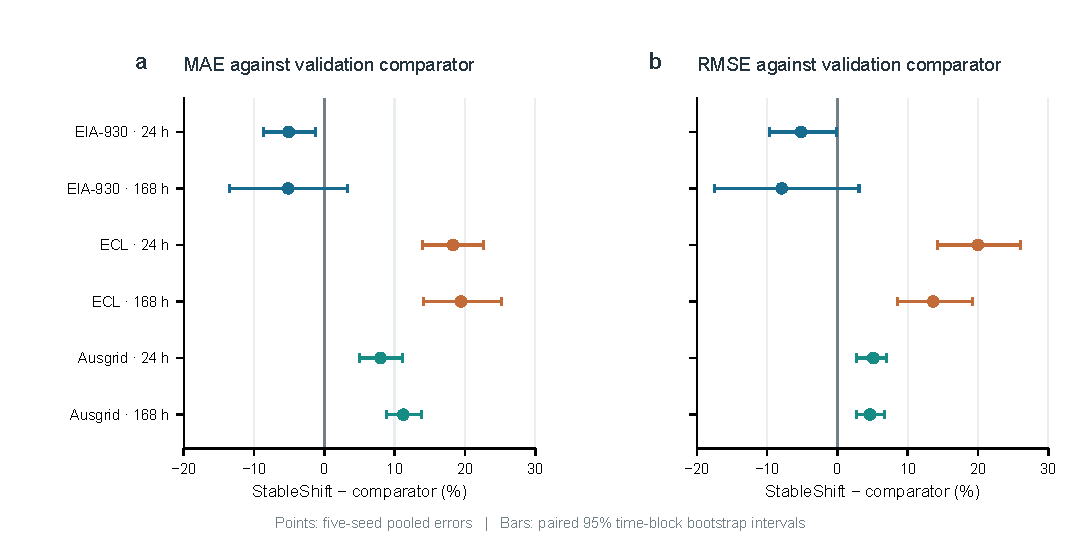
\includegraphics[width=\textwidth]{figures/fig2_accuracy.pdf}
\caption{\textbf{Forecasting gains depend on the data scale.} Paired relative differences in (a) MAE and (b) RMSE from the validation-selected comparator. Negative values favor StableShift. The comparator is TiDE except for ECL 168 h, where it is weekly persistence. Points pool five seeds; bars are pointwise 95\% paired crossed seed/time-block bootstrap intervals with 5,000 resamples. Scheduled origins retain their positions when labels are unavailable. Holm-adjusted tests are reported separately.}
\label{fig:accuracy}
\end{figure*}

The customer and household benchmarks produce a different ordering. Relative to the fixed validation comparators, StableShift's MAE is 18.3--19.4\% higher on ECL and 8.0--11.3\% higher on Ausgrid. TiDE gives the lowest chronological ECL point estimates in Table~\ref{tab:main}, while the best household result varies by metric and horizon. Across the six chronological cells, the equal-cell relative MAE difference is $+7.81\%$ (95\% CI $+5.77$ to $+9.94\%$), and the RMSE difference is $+5.04\%$ ($+2.81$ to $+7.62\%$). This pattern identifies regional demand as the present design's strongest application.

\subsection{Regional accuracy under altered inputs}
On EIA 24 h, StableShift has lower MAE than TiDE in all four perturbed-input conditions. The differences are $-4.46\%$ for missing inputs, $-9.03\%$ for recent amplitude scaling, $-9.96\%$ for affine offset and $-19.67\%$ for block anomalies. The last three contrasts retain Holm-adjusted significance, with adjusted $p=0.012$, $0.049$ and $0.012$, respectively. At 168 h, the corresponding point-estimate advantages are 2.16\%, 8.83\%, 11.24\% and 12.12\%; their multiplicity-adjusted tests are less decisive.

Figure~\ref{fig:stress} shows absolute comparative error alongside degradation from each model's chronological forecast. Under the 24 h block anomaly, StableShift's MAE rises from 1,562 to 1,622 MW, a factor of 1.038, whereas TiDE rises from 1,646 to 2,019 MW, a factor of 1.227. Under missing inputs, StableShift retains lower absolute MAE, with a larger increase relative to its own chronological error.

\begin{figure*}[t]
\centering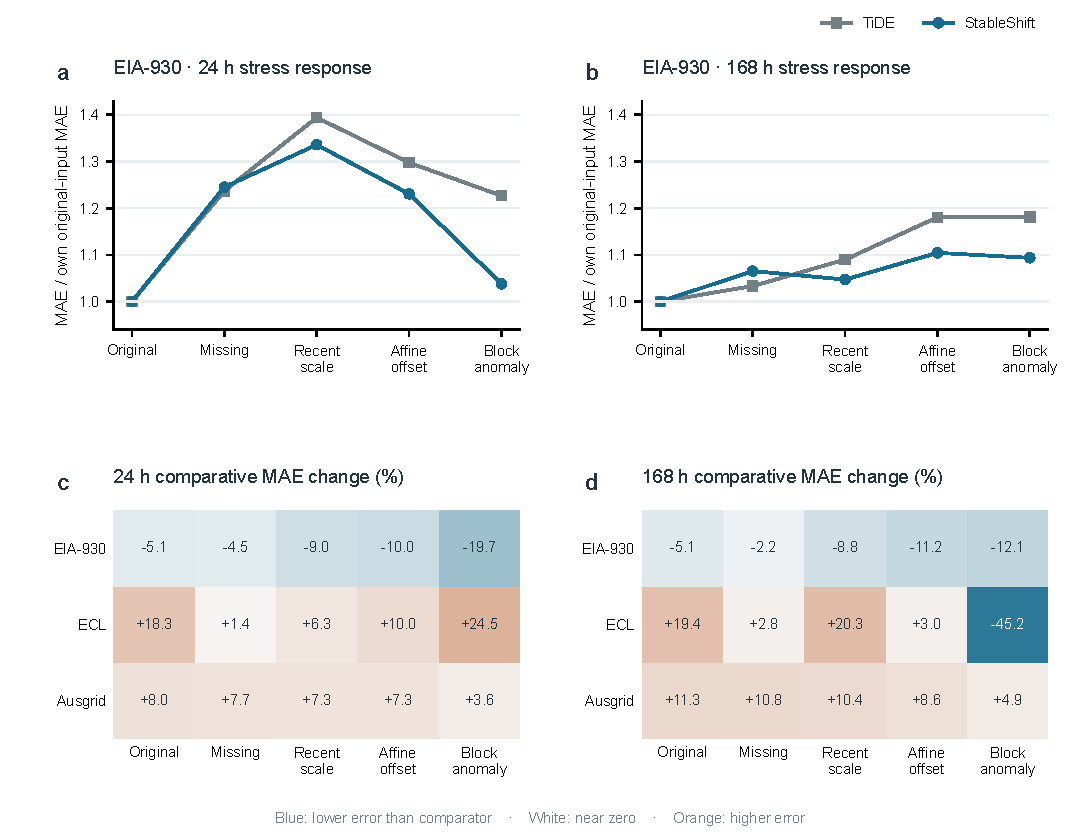
\includegraphics[width=\textwidth]{figures/fig3_input_response.pdf}
\caption{\textbf{Absolute accuracy and degradation describe complementary responses to altered inputs.} (a,b) EIA MAE divided by each method's own chronological MAE, for 24 h and 168 h forecasts. Lines connect categorical conditions for readability and do not represent increasing perturbation severity. (c,d) Relative MAE differences from the fixed validation comparator across all three datasets. Colors and printed values use the same scale; negative values favor StableShift. All conditions alter observed context loads only and retain the original future labels. Values pool five seeds. Pointwise uncertainty and adjusted tests are provided in Supplementary Table S3 and Source Data.}
\label{fig:stress}
\end{figure*}

Across all 30 main data/horizon/input-condition cells, the macro relative difference is $+1.77\%$ in MAE (95\% CI $-0.18$ to $+3.86\%$) and $-0.68\%$ in RMSE ($-2.83$ to $+1.59\%$). The worst-cell MAE difference is $+24.54\%$ ($+18.48$ to $+43.00\%$).

\subsection{Learned corrections dominate the observed EIA gain}
Removing both learned corrections raises EIA MAE from 1,562 to 2,359 MW at 24 h and from 2,573 to 3,051 MW at 168 h. Expressed relative to the anchor-only model, the full forecaster reduces MAE by 33.8\% and 15.7\%. Conversely, removing online updates changes the chronological MAE by only $-0.0015\%$ and $+0.0011\%$ relative to the full model. Across all 30 main conditions, the largest absolute MAE difference from disabling updates is 0.0524\% (Fig.~\ref{fig:components}). The useful regional forecasting behavior is therefore already present in the fitted correction pathways.

The drift gate updates nine of 181 EIA 24 h origins and one of 25 EIA 168 h origins. It makes no updates on the unmodified ECL streams and updates 50 of 219 and five of 31 Ausgrid origins. Reconstruction telemetry characterizes the update activity, complementing the paired forecast comparison. Removing the representation penalties while retaining spectral normalization produces smaller, directionally mixed effects. Input conditioning also has condition-dependent effects, with removal improving the EIA missing-input point estimates. Supplementary Table S4 reports every available five-seed intervention and its uncertainty.

\begin{figure*}[t]
\centering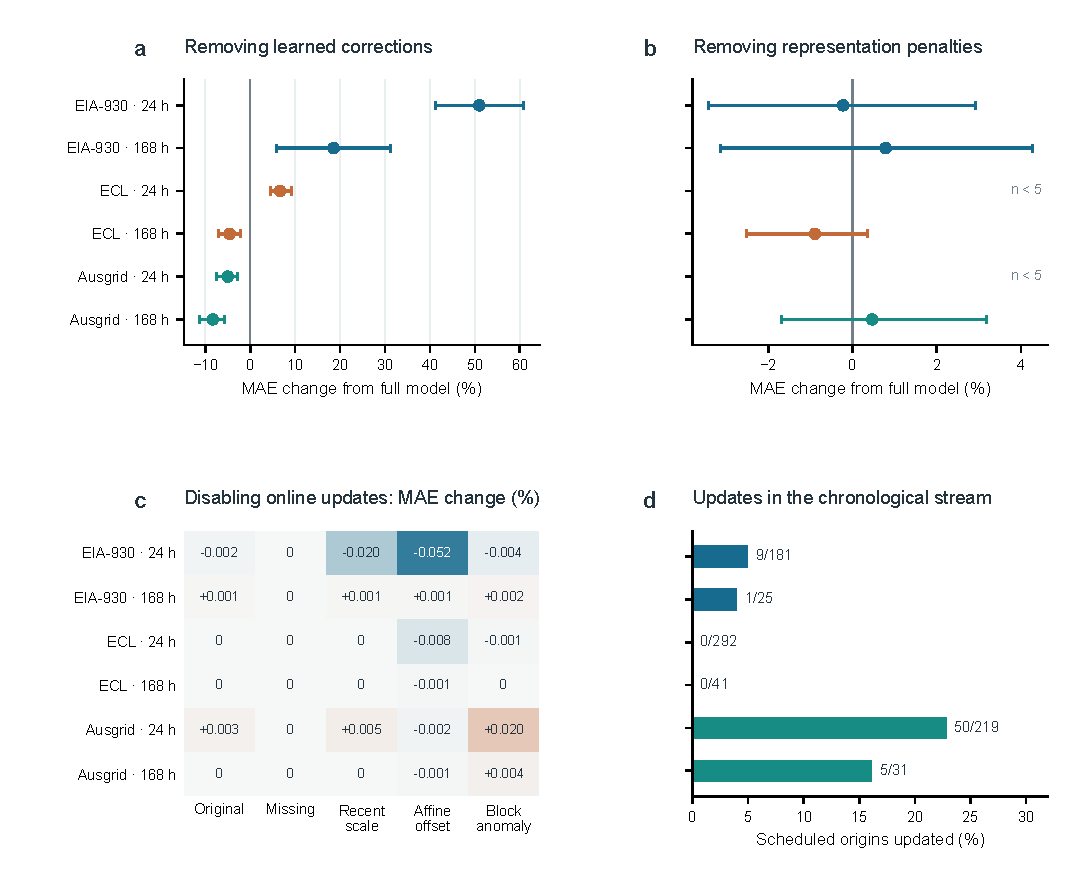
\includegraphics[width=\textwidth]{figures/fig4_components.pdf}
\caption{\textbf{Component interventions locate the source of forecasting performance.} (a) Removing the learned linear and neural corrections, leaving the seasonal reference. (b) Retraining without consistency and representation-energy penalties; spectral normalization and reconstruction remain enabled. Points and bars in (a,b) show relative MAE changes from the full model and pointwise paired 95\% intervals, with five seeds. Cells with fewer than five completed retraining seeds are labeled. (c) The effect of disabling online updates is displayed on its own small numerical scale; values below 0.0005\% in magnitude round to zero. (d) Triggered updates divided by scheduled origins on unmodified input streams. Positive intervention effects mean that the removed component helped the full model.}
\label{fig:components}
\end{figure*}

\subsection{Regional transfer and deployment cost}
The separate three-seed transfer evaluation gives StableShift MAE values of 4,369 MW on ERCO and 2,267 MW on SWPP (Fig.~\ref{fig:transfer}). Relative to validation-selected PatchTST, these are point-estimate reductions of 6.23\% and 11.59\%. The ERCO interval includes zero; complete transfer intervals appear in Supplementary Table S6. DLinear has lower ERCO RMSE, while daily persistence nearly matches StableShift's SWPP MAE. The anchor-only variant has slightly lower MAE on both regions, indicating a substantial contribution from the transferred seasonal reference.

The mutable state contains 2,048 parameters at every horizon. Total model size ranges from 526,560 parameters for EIA 24 h to 978,657 for a 16-channel 168 h model. EIA 24 h median per-origin latency is 4.24 ms on the recorded RTX 4060 Laptop GPU; the measured median includes triggered adaptation at its observed frequency. The corresponding maximum allocated GPU memory during the inference stream is 25.93 MiB. Supplementary computational measurements are grouped by hardware, including V100/V100S archival runs. Figure~\ref{fig:transfer} compares model size and latency within the EIA hardware setting.

\begin{figure*}[t]
\centering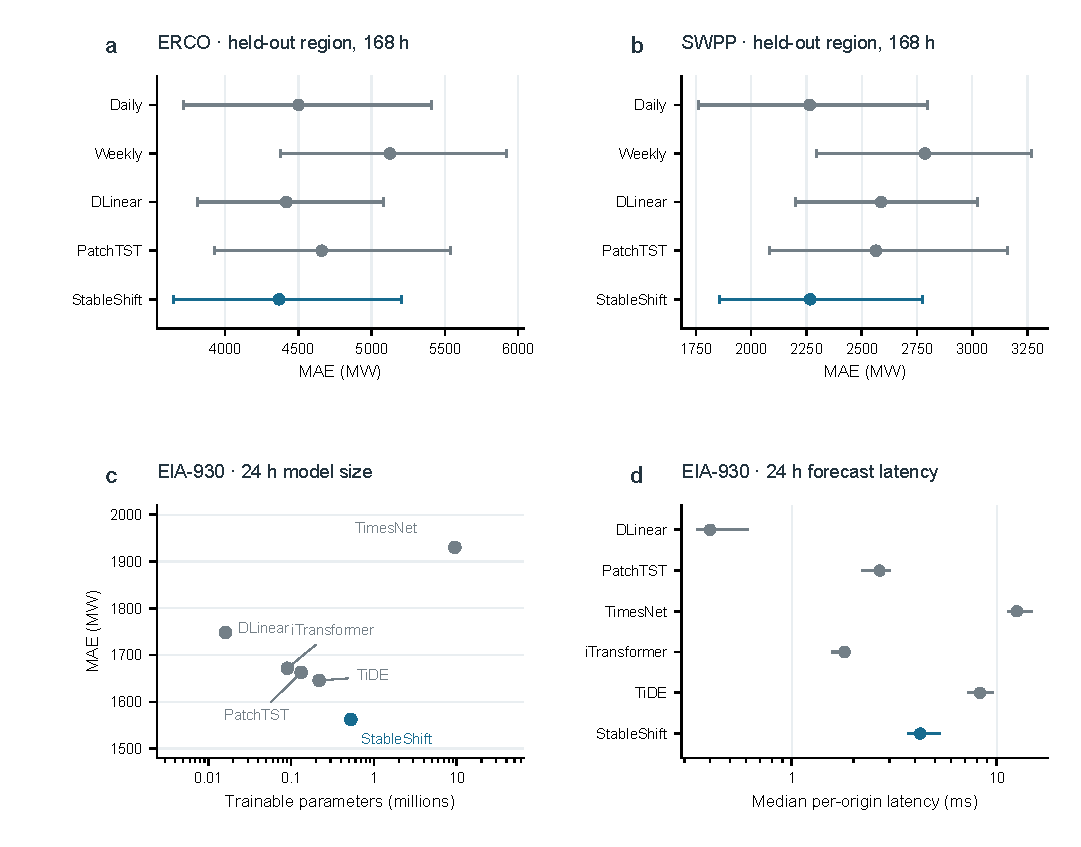
\includegraphics[width=\textwidth]{figures/fig5_transfer_cost.pdf}
\caption{\textbf{Transfer and computation complete the operating profile.} (a,b) Absolute MAE for previously unseen ERCO and SWPP at 168 h, using three seeds; bars show pointwise 95\% crossed seed/weekly-origin bootstrap intervals. Each region has its own horizontal scale. (c) Parameter count and chronological EIA 24 h MAE for the completed neural methods. (d) Median EIA 24 h latency on the same RTX 4060 Laptop GPU. Points are medians across the five seed-specific latency medians; lines span their minimum and maximum, not confidence intervals. Logarithmic axes are used for parameter count and latency. Measured forecasting time includes the online update when it is triggered.}
\label{fig:transfer}
\end{figure*}

\section{Discussion}
Anchored forecasting turns recurring demand structure into an explicit reference for learning. On the recent EIA-930 holdout, the fitted corrections improve day-ahead accuracy and sustain an advantage under the specified altered-input conditions. The joint correction intervention identifies these pathways as the main source of the regional gain. The seasonal reference thus provides both a useful forecasting foundation and an interpretable baseline for measuring what the model learns.

The compact online state adds a separately controlled deployment mechanism. Factor projection and the sensitivity proposition link the update budget to forecast displacement; paired deployment streams quantify its marginal accuracy effect. Together, they make online modification mathematically explicit and empirically measurable. This component-level perspective complements recent shift-aware and test-time learning methods \cite{kim2025tta,apt2026,adanodes2026,adamshift2026} and motivates closer alignment between reconstruction and the forecasting objective.

The cross-scale pattern identifies regional demand as the clearest application of the present design and makes the seasonal reference a useful focus for further architectural study. The evaluation covers hourly public-load data, horizons up to one week and the specified input perturbations. By combining a recent operating-data holdout with matched interventions, the study connects forecast accuracy to its source and provides a practical basis for improving persistent representations and online learning independently.

\section{Conclusion}
StableShift establishes an explicit architecture for anchored forecasting with a small, controlled online state. On the January--June 2026 EIA-930 holdout, its learned corrections deliver useful day-ahead accuracy and strong responses to the specified amplitude and anomaly perturbations. The low-rank pathway adds a mathematically characterized interface for label-free modification, and matched interventions identify where its contribution enters. Together, the architecture, recent regional evidence and component-level analysis provide a concrete foundation for developing electricity-demand forecasters whose persistent knowledge and online learning can be improved independently.

\section*{Data availability}
EIA-930, ECL and Ausgrid are publicly accessible from the sources cited in this article. Prepared-data identifiers, exact observation periods, channel selections, transformations and split definitions are supplied with the reproducibility files. Source Data accompanying this manuscript contain the aggregate results, seed-level metrics, paired comparisons, computational measurements and reference-verification records. Original datasets remain subject to their providers' terms.

\section*{Code availability}
Source code, configurations, environment records, data-preparation instructions and manuscript-generation scripts are publicly available at \url{https://github.com/bianyanbo44-afk/stable-shift-forecasting}. Release v0.1.0 provides the completed forecast streams, run records and source snapshots. Run manifests link each reported analysis to its saved predictions.

\section*{CRediT authorship contribution statement}
Yanbo Bian: Conceptualization, Methodology, Software, Validation, Formal analysis, Investigation, Data curation, Visualization, Writing---original draft, Writing---review and editing.

\section*{Funding}
This research received no specific grant from any funding agency in the public, commercial, or not-for-profit sectors.

\section*{Declaration of competing interest}
The author declares no competing financial interests or personal relationships that could have influenced the work reported in this paper.

\section*{Declaration of generative AI and AI-assisted technologies}
OpenAI Codex assisted with software development, analysis scripting, manuscript drafting and editing, and programmatic figure preparation. Numerical results were calculated from saved experimental outputs. AI assistance is disclosed as a tool contribution and does not constitute authorship.

\section*{Supplementary material}
Supplementary Information provides the sensitivity proof, full data and implementation specifications, paired statistical results, all available secondary experiments and reproducibility details. The accompanying Source Data are machine-readable.

\setlength{\bibsep}{2pt plus 0.5pt minus 0.5pt}
\bibliographystyle{elsarticle-num}
\bibliography{references}
\end{document}
